\section{History}
\label{sec:history}
Throughout history, questions surrounding the origin, age, and size of the universe have fascinated humans. Plato believed in a Universe that remains constant, envisioning it as an entity that was created perfect, unaging, and free from decay \citep{cornford_platos_2010}. This view of a static universe prevailed for more than two millennia, and it was so entrenched in cosmological thinking that even Albert Einstein initially subscribed to it. To reconcile his field equations of general relativity with the notion of a static universe, Einstein introduced the cosmological constant, a term that provided a mathematical means to allow for static solutions to his equations \citep{einstein_kosmologische_1917}.

However, the early 20th century brought discoveries that challenged the long-standing paradigm of a static universe. Vesto Slipher made pivotal observations, noting that most galaxies recede from the Milky Way at high velocities. Building on this foundation, Edwin Hubble, in the 1920s, conducted an analysis of the escape velocities of distant galaxies, leading to a groundbreaking discovery. Hubble observed that the farther away galaxies are, the faster they appear to be moving away. He plotted the radial velocities of these galaxies against their distances and found that the data could be best described by a straight line, indicating a linear relationship (\cref{fig:hubble}).

\begin{figure}
    \centering
    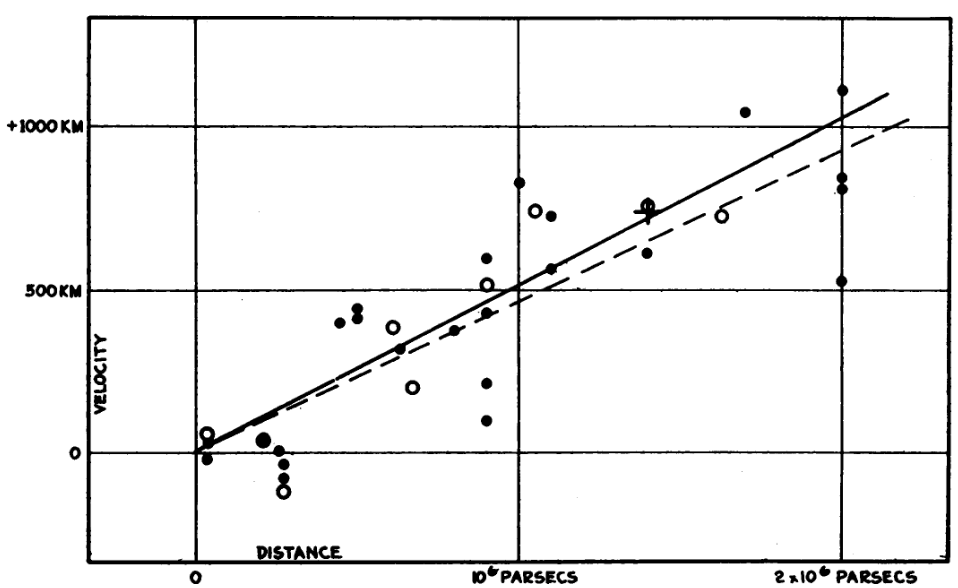
\includegraphics[width=0.8\linewidth, keepaspectratio]{img//chapter1/hubble.png}
    \caption[Hubble's Law: radial velocities of Extra-Galactic Nebulae]{Radial velocities, corrected for solar motion, plotted against distances estimated from involved stars and mean luminosities of nebulae in a cluster.\\\small{Credits: \cite{hubble_relation_1929}.}}
    \label{fig:hubble}
\end{figure}

Hubble's choice of a linear fit was influenced by his belief in the predictions of Friedmann's equations, which are solutions to Einstein's field equations of general relativity and suggest an expanding universe. Hubble's analysis and the linear relationship he identified, the basis for what is now known as \emph{Hubble's Law}, marked a fundamental shift in the understanding of the universe. It provided strong evidence for an expanding Universe, a concept that fundamentally contradicted the long-held belief in a static cosmos. This discovery not only revolutionized cosmology, but also led Einstein to reconsider the cosmological constant he had introduced.

The receding velocity $v$ of a galaxy leads to a Doppler shift in the galaxy's spectrum, observable as a redshift $z$:
\be
\label{eq:1.1}
v (r) = c \frac{\D \l}{\l} = c z = H_0 r \,,
\ee
where $H_0$ is the proportionality constant, subsequently named after Hubble, for which, in 1929 he published \citep{hubble_relation_1929} a value of
\be
\label{eq:1.2}
H_0 = \SI{530}{\kilo\meter\per\second\per\mega\parsec} \,,
\ee
much different from the current value \citep{tully_hubble_2023} of
\be
\label{eq:1.3}
H_0 = \SI[separate-uncertainty=true]{74.6 \pm 0.8}{\kilo\meter\per\second\per\mega\parsec} \,.
\ee

The unit of the Hubble constant is chosen according to the relation between escape velocity and
distance, but actually it has the unit of an inverse time, representing the age of the universe in a uniformly expanding model:
\be
\label{eq:1.4}
\tau_0 = H_0^{-1} \approx 13.9\pwr{9} \si{\year} \,.
\ee